\documentclass{article}
\usepackage{graphicx} % Required for inserting images
\usepackage[utf8]{inputenc}
\usepackage{polski}
\usepackage[dvipsnames]{xcolor}
\usepackage{indentfirst}
\usepackage{multicol}
\usepackage{geometry}
\usepackage{titlesec}
\usepackage[colorlinks=true, linkcolor=gray, urlcolor=blue, citecolor=green]{hyperref}
\usepackage{makecell}
\usepackage{float}
\usepackage[polish]{babel}
\usepackage[T1]{fontenc}
\usepackage[justification=centering]{caption}
\usepackage[utf8]{inputenc} 
\usepackage{subfig}


\usepackage{mwe} % for 'example-image'
\usepackage{newfloat}
\DeclareFloatingEnvironment{graph}
\addto\captionspolish{%
  \renewcommand{\graphname}{Wykres}%
  \renewcommand{\figurename}{Rysunek}%
  \renewcommand{\tablename}{Tabela}%
}


\begin{document}

\begin{titlepage}
    \begin{center}
        \vspace*{1cm}
            
        \Huge
        \textbf{Sprawozdanie z laboratorium 6}
            
        \vspace{0.5cm}
        \LARGE
        HART (WAGO)
            
        \vspace{1.5cm}
            
        \textbf{Łukasz Janusz\\Marek Generowicz}

        \normalsize      
        \textcolor{gray}{09.03.2025}
        \vfill
        \begin{figure}[hb]
            \centering
            
\includegraphics[width=0.5\textwidth]{media/Logo_AGH.jpg}
        \end{figure}   
    \end{center}
\end{titlepage}

\section{Wstęp}
Na laboratoriach należało zapoznać się z protokołem HART, zasadami komunikacji oraz praktycznymi aspektami wykorzystania go w przemyśle. W trakcie zajęć przeprowadzono ćwiczenia z wykorzystaniem sterownika \textit{WAGO 750-841} wyposażonym w dwukanałowy analogowy moduł wejścia, który pozwala na komunikację z urządzeniami HART. Elementem pomiarowym natomiast jest \textit{termopara typu K}, która została połączona z modułem WAGO za pomocą przetwornika temperatury \textit{TxIsoRail-HART}. 
\subsection{Protokół HART}
Protokół HART \textit{(High Addressable Remote Transducer)} jest standardem komunikacyjnym stosowanym w przemyśle, który pozwala na komunikację z urządzeniami pomiarowymi, takimi jak czujniki, przetworniki, zawory, itp. Protokół HART umożliwia przesyłanie danych cyfrowych i analogowych w jednym przewodzie. Komunikacja odbywa się za pomocą sygnałów modulowanych na sygnale prądu stałego, co pozwala na przesyłanie danych cyfrowych wraz z sygnałem analogowym. Protokół HART jest kompatybilny z większością urządzeń pomiarowych, co pozwala na łatwe wdrożenie w istniejących systemach. Urządzenia, które wykorzystują protokół HART, są podzielone na nadrzędne (np. sterowniki PLC) i podrzędne (np. czujniki).

\section{Przebieg ćwiczenia}

\subsection{Konfiguracja PLC}
W pierwszej części zadania należało zaprogramować sterownik \textit{WAGO}. W tym celu należało skorzystać z aplikacji \textit{CoDeSys}. Ważne aby w nowo stworzonym projekcie ustawić \textit{Type od POU} na \textit{Program} a język programowania na \textit{FBD} ze względy na konieczność wykorzystania biblioteki do obsługi \textit{POU} napisanej w tym właśnie języku. Następnie należało dodać moduły wejścia i wyjścia w wirtualnym wnętrzu magistrali. Uzupełniona magistrala wyglądała jak na rysunku \ref{fig1}.

\vspace{1em}
\begin{figure}[ht]
    \centering
    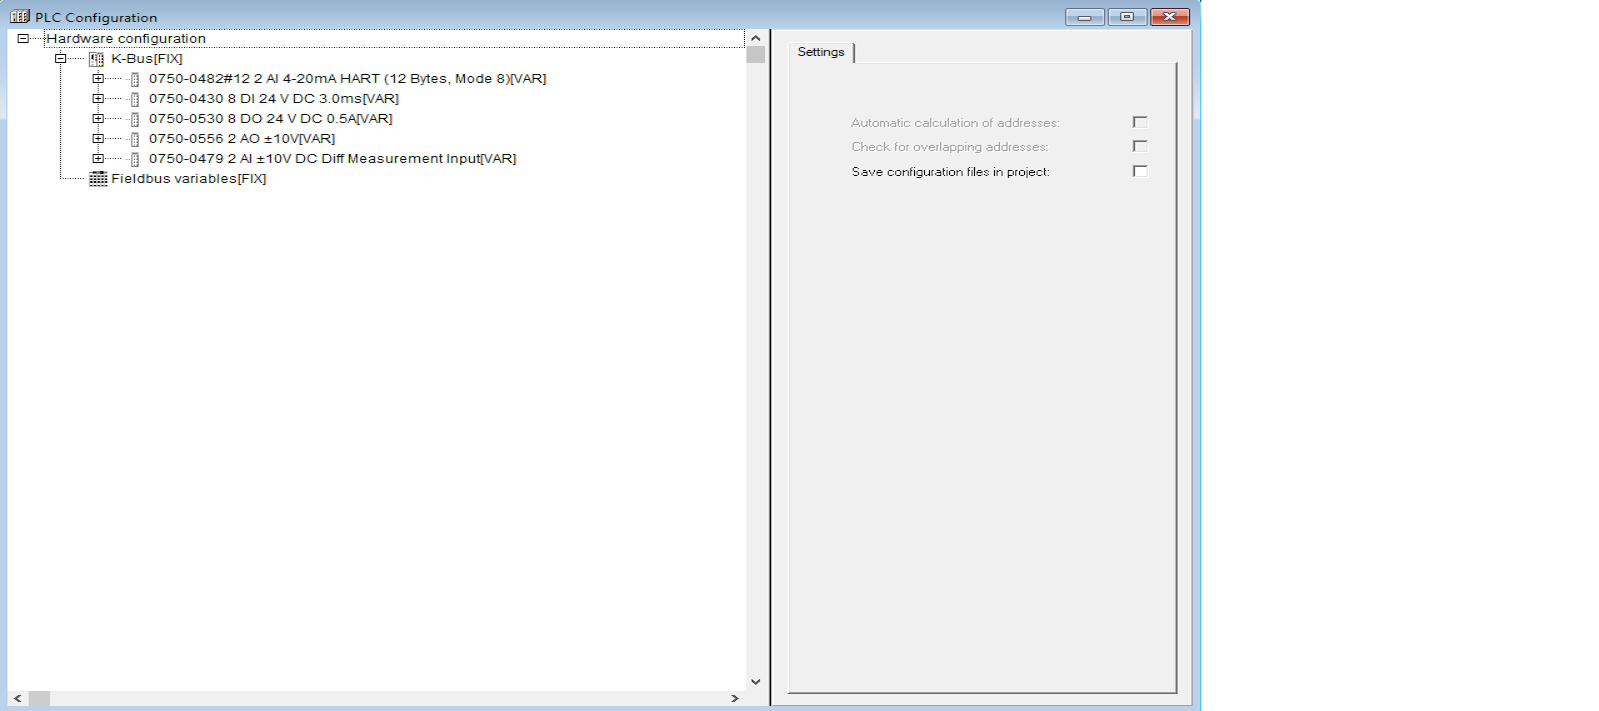
\includegraphics[width=1.3\linewidth]{media/6.png}
    \caption{Wnętrze magistrali w aplikacji \textit{CoDeSys}.}
    \label{fig1}
\end{figure}

Przed przystąpieniem do programowania należało skonfigurować parametry komunikacji oraz, w razie gdyby jej nie było, dodać bibliotekę do obsługi komunikacji HART \textit{WagoLibHART\_03.lib}
\newpage


\subsection{Program - HART\_INFO} \label{1a}

\subsection{Program - odczyt zmiennych HART}

\subsection{Dane HART}
W celu sprawdzenia ilości zmiennych dynamicznych skorzystaliśmy z  tabeli z dokumentacji urządzenia. 
\begin{table}[H]
    \centering
    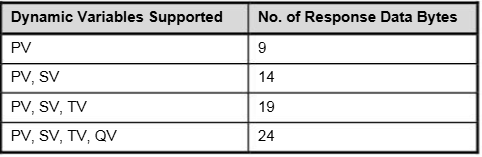
\includegraphics{media/Tabela_z_dokumentacji.png}
    \caption{Tabela z dokumentacji}
\end{table}
Aby tabela była użyteczna sprawdziliśmy wartość pola CMD3.bCmdDataCount, którego wartość wynosi 19. Dzięki temu wiemy, że nasze urządzenie obsługuje dokładnie 3 zmienne dynamiczne. 

\begin{figure}[H]
    \centering
    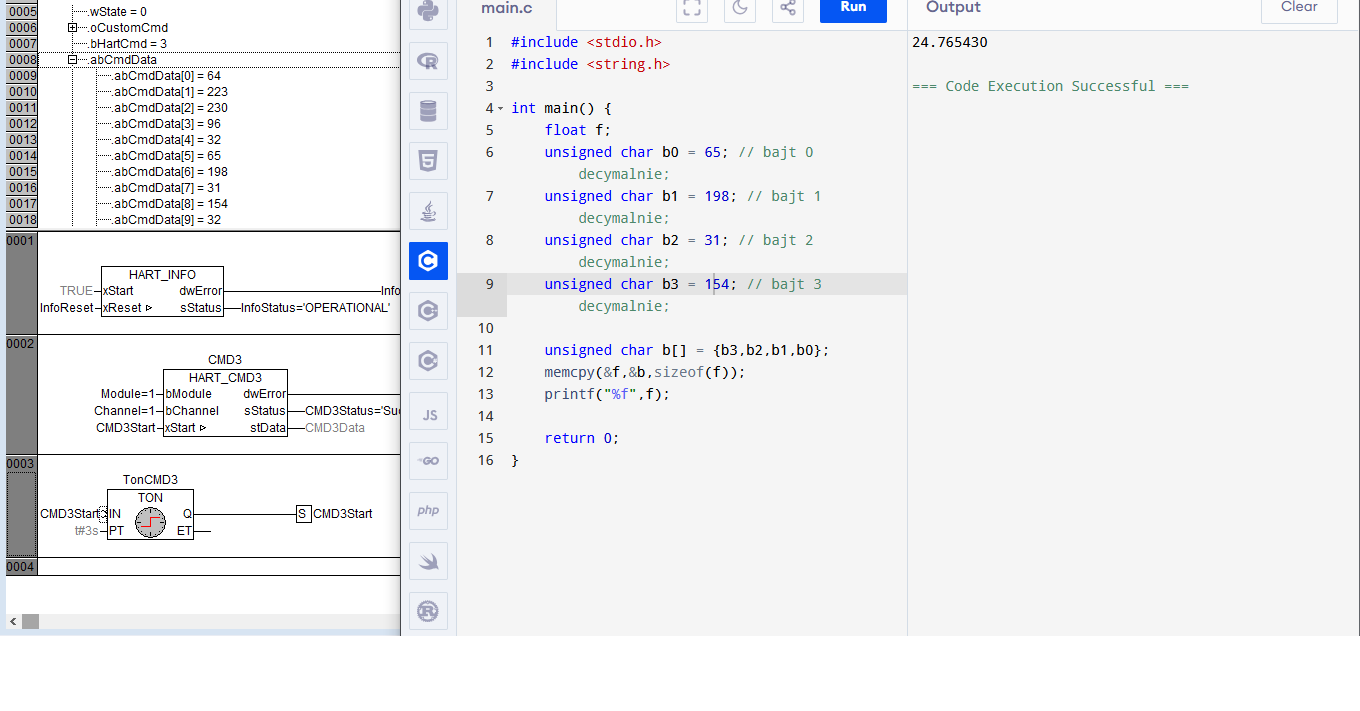
\includegraphics[width=1\linewidth]{media/7.png}
    \caption{Wartości poszczególnych pól adCmdData wraz z ich sprawdzeniem z użyciem języka C}
\end{figure}

\end{document}
